\documentclass{article} 

\usepackage[brazil]{babel}
\usepackage{enumitem}
\usepackage{amsmath}
\usepackage{booktabs}
\usepackage{bm}
\usepackage{float}
\usepackage[margin=2cm]{geometry}
\usepackage{circuitikz}
\usepackage{siunitx}
\usepackage{steinmetz}
\usepackage{amssymb}

\newcommand{\phasor}[2]{%
  #1 \, \phase{\, #2^\circ} \,
}

\newcommand{\ds}{\displaystyle}

% \newcommand{\phasor}[2]{%
%   #1 \, \text{\phase{\, \ang{#2}}} \,
% }

\newcommand{\nle}{%
  \notag \\[0pt]
}

\setlength{\parindent}{0pt}

\title{Modelagem Matemática da Microrrede CC} 
\author{} 
% \date{\today}
\date{}

\begin{document}

\maketitle

% \section*{Esquemático da Microrrede CC}

% \begin{figure}[h]
%   \centering
%   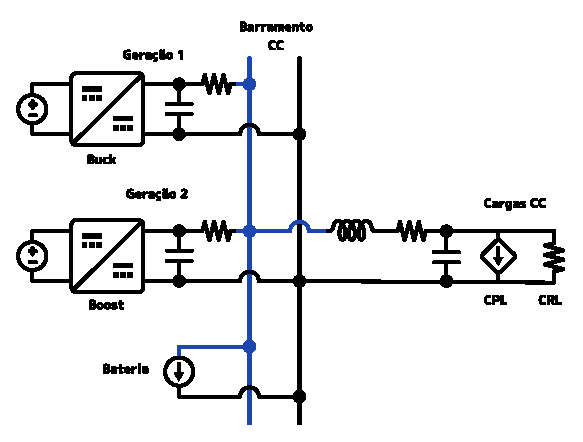
\includegraphics[width=14cm]{assets/dc_microgrid.eps}
%   \caption{Esquemático da Microrrede CC}
%   \label{fig:exemplo}
% \end{figure}


\section*{Modelo Não-linear da Microrrede CC}

\subsection*{Modelagem do Subsistema: Geração 1}

O sistema da geração 1, apresentado na Figura~\ref{fig:subsystem_1},  é composto por uma fonte de alimentação cuja tensão varia ao longo do tempo, a qual está conectada a um conversor do tipo {\it buck}. Este conversor, por sua vez, está ligado a um filtro RC. Finalmente, o conjunto é conectado ao barramento de corrente contínua (CC).

\begin{figure}[H]
  \centering
  \begin{circuitikz}[american, scale=0.5, font=\footnotesize]
    \ctikzset{bipoles/length=1cm}
    \draw
    (0,4) to[vsource, v_=$v_{\text{in}, 1}(t)$] (0,0)
    (0,4) to[normal open switch, l=$S_1$] (4,4)
    (4,0) to[diode, l=$D_1$] (4,4)
    (4,4) to[L, l=$L_1$, i_=$i_{L,1}(t)$] (8,4)
    (7,4) to[R, l=$R_{1,1}$] (11,4)
    (11,4) to[C, l=$C_1$, v=$v_{C,1}(t)$] (11,0)
    (11,4) to[R, l=$R_{1,2}$, i_=$i_{E,1}(t)$] (15,4)

    (15,4) to[short, -o] (16,4)
    (0,0) to[short, -o] (16,0)

    (16,4) to[open, v=$v_E(t)$] (16,0)
    ;
  \end{circuitikz}
  \caption{Circuito elétrico do sistema da geração 1.}
  \label{fig:subsystem_1}
\end{figure}

Aplicando a LKT na segunda malha a partir da esquerda, obtemos:
\begin{gather}
  d_1(t) v_{\text{in}, 1} - L_1 \dot{i}_{L,1} - R_{1,1} i_{L,1}(t) - v_{C,1}(t) = 0 \nle
  \dot{i}_{L,1} = - \frac{R_{1,1}}{L_1} i_{L,1}(t) - \frac{1}{L_1} v_{C,1}(t) + \frac{v_{\text{in}, 1}}{L_1} d_1(t)
\end{gather}

Aplicando a LKC, obtemos:
\begin{gather}
  i_{L,1}(t) = C_1 \dot{v}_{C,1} + i_{E,1}(t)
\end{gather}

Têm-se que, $i_{E,1}(t) = \ds \frac{v_{C,1}(t) - v_E(t)}{R_{1,2}}$. Logo,
\begin{gather}
  i_{L,1}(t) = C_1 \dot{v}_{C,1} + \frac{1}{R_{1,2}}v_{C,1}(t) - \frac{1}{R_{1,2}} v_E(t) \nle
  i_{L,1}(t) = C_1 \dot{v}_{C,1} + \frac{1}{R_{1,2}}v_{C,1}(t) - \frac{1}{R_{1,2}} v_E(t) \nle
  \dot{v}_{C,1} = \frac{1}{C_1} i_{L,1}(t) - \frac{1}{R_{1,2}C_1 }v_{C,1}(t) + \frac{1}{R_{1,2} C_1} v_E(t)
\end{gather}

Portanto, o modelo do subsistema da geração é:
\begin{gather}
  \begin{cases}
    \dot{i}_{L,1} = \ds - \frac{R_{1,1}}{L_1} i_{L,1}(t) - \frac{1}{L_1} v_{C,1}(t) + \frac{v_{\text{in}, 1}}{L_1} d_1(t) \\[12pt]
    \dot{v}_{C,1} = \ds \frac{1}{C_1} i_{L,1}(t) - \frac{1}{R_{1,2}C_1 }v_{C,1}(t) + \frac{1}{R_{1,2} C_1} v_E(t)
  \end{cases}
\end{gather}

\vspace*{8pt}
\subsection*{Modelagem do Subsistema: Conversor Boost}

O sistema da geração 2, apresentado na Figura~\ref{fig:subsystem_2},  é composto por uma fonte de alimentação cuja tensão varia ao longo do tempo, a qual está conectada a um conversor do tipo {\it boost}. Este conversor, por sua vez, está ligado a um filtro RC. Finalmente, o conjunto é conectado ao barramento de corrente contínua (CC).

\begin{figure}[H]
  \centering
  \begin{circuitikz}[american, scale=0.5, font=\footnotesize]
    \ctikzset{bipoles/length=1cm}
    \draw
    (-4,4) to[vsource, v_=$v_{\text{in}, 2}(t)$] (-4,0)
    (-4,4) to[R, l=$R_{2,1}$, i_=$i_{L,2}$] (0,4)
    (0,4) to[L, l=$L_2$] (4,4)
    (4,0) to[normal open switch, l=$S_2$] (4,4)
    (4,4) to[diode, l=$D_2$] (8,4)
    (8,4) to[C, v=$v_{C,2}$, l=$C_2$] (8,0)
    (8,4) to[R, l=$R_{2,2}$, -o, i=$i_{E,2}$] (12,4)
    (-4,0) to[short, -o] (12,0)
    (12,4) to[open, v=$v_E$] (12,0)
    ;
  \end{circuitikz}
  \caption{Circuito elétrico do sistema da geração 2.}
  \label{fig:subsystem_2}
\end{figure}

\subsubsection*{Para $S_2$ fechada: $d_2(t) \cdot T_s$}

Aplicando a LKT na malha mais a esquerda, obtemos:
\begin{gather}
  v_{\text{in}, 2}(t) - R_{2,1} i_{L,2}(t) - L_2 \dot i_{L,2} = 0  \nle
  \dot i_{L,2} = - \frac{R_{2,1}}{L_2} i_{L,2}(t) + \frac{1}{L_2} v_{\textit{in}, 2}
\end{gather}

Aplicando a LKC na malha mais a direita, tém-se:
\begin{gather}
  i_{E,2}(t) + C_2 \dot{v}_{C,2} = 0
\end{gather}

Como $i_{E,2}(t) = \ds \frac{v_{C,2}(t) - v_E(t)}{R_{2,2}}$, têm-se:
\begin{gather}
  \frac{v_{C,2}(t)}{R_{B,2}} - \frac{v_E(t)}{R_{B,2}} + C_2 \dot{v}_{C,2} = 0 \nle
  \dot{v}_{C,2} = - \frac{1}{R_{B,2} C_2} v_{C,2}(t) + \frac{1}{R_{B,2} C_2} v_{E}(t)
\end{gather}

Assim, neste modo, têm-se:
\begin{gather}
  \begin{cases}
    \dot i_{L,2} = \ds - \frac{R_{2,1}}{L_2} i_{L,2}(t) + \frac{1}{L_2} v_{\textit{in}, 2} \\[12pt]
    \dot{v}_{C,2} = \ds - \frac{1}{R_{B,2} C_2} v_{C,2}(t) + \frac{1}{R_{B,2} C_2} v_{E}(t)
  \end{cases}
\end{gather}

\vspace*{8pt}
\subsubsection*{Para $S_2$ aberta: $\left[1 - d_2(t)\right] \cdot T_s$}

Aplicando a LKT, obtemos:
\begin{gather}
  v_{\text{in}, 2}(t) - L_2 \dot i_{L,2} - R_{2,1} i_{L,2} (t) - v_{C,2} (t)= 0 \nle
  \dot i_{L,2} = - \frac{R_{2,1}}{L_2} i_{L,2}(t) - \frac{1}{L_2} v_{C,2}(t) + \frac{1}{L_2} v_{\text{in}, 2}
\end{gather}

Aplicando a LKC, obtemos:
\begin{gather}
  i_{L,2}(t) = C_2 \dot v_{C,2} + i_{E,2}(t) \nle
  i_{L,2}(t) = C_2 \dot v_{C,2} +  \frac{v_{C,2}(t)}{R_{2,2}} - \frac{v_E(t)}{R_{2,2}} \nle
  \dot{v}_{C,2} =  \frac{1}{C_2} i_{L,2}(t) - \frac{1}{R_{2,2}C_2} v_{C,2}(t) + \frac{1}{R_{2,2} C_2} v_E(t)
\end{gather}

Assim, neste modo, têm-se:
\begin{gather}
  \begin{cases}
    \dot i_{L,2} = \ds - \frac{R_{2,1}}{L_2} i_{L,2}(t) - \frac{1}{L_2} v_{C,2}(t) + \frac{1}{L_2} v_{\text{in}, 2} \\[12pt]
    \dot{v}_{C,2} = \ds \frac{1}{C_2} i_{L,2}(t) - \frac{1}{R_{2,2}C_2} v_{C,2}(t) + \frac{1}{R_{2,2} C_2} v_E(t)
  \end{cases}
\end{gather}

\vspace*{8pt}
\subsubsection*{Modelo Médio Completo}
A equação completa da dinâmica da corrente ${i}_{L,2}(t)$ é:
\begin{gather}
  \dot{i}_{L,2} = \left[- \frac{R_{2,1}}{L_2} i_{L,2}(t) + \frac{1}{L_2} v_{\textit{in}, 2}\right] d_2(t) + \left[- \frac{R_{2,1}}{L_2} i_{L,2}(t) - \frac{1}{L_2} v_{C,2}(t) + \frac{1}{L_2} v_{\text{in}, 2}(t)\right] \left[1 - d_2(t)\right] \nle
  \dot{i}_{L,2} = - \frac{R_{2,1}}{L_2} i_{L,2}(t) - \frac{1}{L_2} v_{C,2}(t) \left[1 - d_2(t)\right] + \frac{1}{L_2} v_{\text{in}, 2}(t)
\end{gather}

E da tensão,
\begin{gather}
  \dot{v}_{C,2} = \left[- \frac{1}{R_{B,2} C_2} v_{C,2}(t) + \frac{1}{R_{B,2} C_2} v_{E}(t)\right] d_2(t) + \left[\frac{1}{C_2} i_{L,2}(t) - \frac{1}{R_{2,2} C_2} v_{C,2}(t) + \frac{1}{R_{2,2} C_2} v_E(t)\right] \left[1 - d_2(t)\right] \nle
  \dot{v}_{C,2} = \frac{1}{C_2} i_{L,2}(t) \left[1 - d_2(t)\right] - \frac{1}{R_{2,2} C_2} v_{C,2}(t) + \frac{1}{R_{2,2} C_2} v_E(t)
\end{gather}

Portanto, o modelo dinâmico do sistema da geração 2 é:
\begin{gather}
  \begin{cases}
    \dot{i}_{L,2} =\ds - \frac{R_{2,1}}{L_2} i_{L,2}(t) - \frac{1}{L_2} v_{C,2}(t) \left[1 - d_2(t)\right] + \frac{1}{L_2} v_{\text{in}, 2} \\[12pt]
    \dot{v}_{C,2} =\ds \frac{1}{C_2} i_{L,2}(t) \left[1 - d_2(t)\right] - \frac{1}{R_{2,2} C_2} v_{C,2}(t) + \frac{1}{R_{2,2} C_2} v_E(t)
  \end{cases}
\end{gather}

\vspace*{8pt}
\subsection*{Modelagem do Subsistema: Cargas}

O circuito que representa as duas cargas conectadas a redes, a CPL e a CRL, é:

\begin{figure}[H]
  \centering
  \begin{circuitikz}[american, scale=0.5, font=\footnotesize]
    \ctikzset{bipoles/length=1cm}
    \draw
    (0,4) to[open, v_=$v_E(t)$, o-o] (0,0)
    (0,4) to[L,l=$L_{K}$, i_=$i_{L_K}(t)$] (4,4)
    (3,4) to[R,l=$R_{K}$] (7,4)
    (7,4) to[C, l=$C_{K}$, v=$v_{C_K}(t)$] (7,0)
    (11,4) to[controlled current source, l={$i(t) = \frac{P_{cpl}(t)}{v_{C_K}(t)}$}] (11,0)
    (0,0) to[short] (16,0)
    (7,4) to[short] (16,4)
    (16,4) to[R, l=$R_{rcl}$] (16,0)
    ;
  \end{circuitikz}
\end{figure}

Aplicando a LKT na malha mais a esquerda, têm-se:
\begin{gather}
  v_E(t) - L_K \dot{i}_{L_K} - R_K i_{L_K}(t) - v_{C_K}(t) = 0 \nle
  \dot{i}_{L_K} = - \frac{R_K}{L_K} i_{L_K}(t) - \frac{1}{L_K} v_{C_K}(t) + \frac{1}{L_K} v_E(t)
\end{gather}

Aplicando a LKC, obtemos:
\begin{gather}
  i_{L_K} = C_K \dot{v}_{C_K} + \frac{P_{cpl}(t)}{v_{C_K}(t)} + \frac{v_{C_K}(t)}{R_{crl}} \nle
  \dot{v}_{C_K} = \frac{1}{C_K} i_{L_K} - \frac{1}{R_{crl} C_K} v_{C_K}(t) - \frac{1}{C_K} \frac{P_{cpl}(t)}{v_{C_K}(t)}
\end{gather}

Portanto, o modelo dinâmico do subsistema das cargas é:
\begin{gather}
  \begin{cases}
    \dot{i}_{L_K} = \ds - \frac{R_K}{L_K} i_{L_K}(t) - \frac{1}{L_K} v_{C_K}(t) + \frac{1}{L_K} v_E(t) \\[12pt]
    \dot{v}_{C_K} = \ds \frac{1}{C_K} i_{L_K} - \frac{1}{R_{crl} C_K} v_{C_K}(t) - \frac{1}{C_K} \frac{P_{cpl}(t)}{v_{C_K}(t)}
  \end{cases}
\end{gather}

\subsection*{Centralização dos Modelos}

Do esquemático, têm-se que:
\begin{gather}
  i_{E,1}(t) + i_{E,2}(t) = i_B(t) + i_{L_K}(t) \nle
  \frac{1}{R_{1,2}} v_{C,1}(t) - \frac{1}{R_{1,2}} v_E(t) + \frac{1}{R_{2,2}} v_{C,2}(t) - \frac{1}{R_{2,2}} v_E(t) =
  i_B(t) + i_{L_K}(t) \nle
  R_{2,2} v_{C,1}(t) - R_{2,2} v_E(t) + R_{1,2} v_{C,2}(t) - R_{1,2} v_E(t) = R_{1,2} R_{2,2} \left[i_B(t) + i_{L_K}(t)\right] \nle
  R_{2,2} v_{C,1}(t) + R_{1,2} v_{C,2}(t) - \left(R_{1,2} + R_{2,2}\right) v_E(t) = R_{1,2} R_{2,2} \left[i_B(t) + i_{L_K}(t)\right]
\end{gather}
\begin{gather}
  v_E(t) = \frac{R_{2,2}}{R_{1,2} + R_{2,2}} v_{C,1}(t) + \frac{R_{1,2}}{R_{1,2} + R_{2,2}} v_{C,2}(t) - \frac{R_{1,2} R_{2,2}}{R_{1,2} + R_{2,2}} \left[i_B(t) + i_{L_K}(t)\right] \nle
  v_E(t) = \frac{R_E}{R_{1,2}} v_{C,1}(t) + \frac{R_E}{R_{2,2}} v_{C,2}(t) - R_E i_B(t) - R_E i_{L_K}(t)
\end{gather}


onde, $R_E = \ds \frac{R_{1,2}R_{2,2}}{R_{1,2} + R_{2,2}}$.

\vspace*{8pt}

Reescrevendo a equação de $i_{L_K}$, obtêm-se:
\begin{gather}
  \dot{i}_{L_K} =  - \frac{R_K}{L_K} i_{L_K}(t) - \frac{1}{L_K} v_{C_K}(t) + \frac{1}{L_K} \left[\frac{R_E}{R_{1,2}} v_{C,1}(t) + \frac{R_E}{R_{2,2}} v_{C,2}(t) - R_E i_B(t) - R_E i_{L_K}(t)\right] \nle
  \dot{i}_{L_K} =  - \frac{R_K + R_E}{L_K} i_{L_K}(t) - \frac{1}{L_K} v_{C_K}(t) + \frac{R_E}{R_{1,2} L_K} v_{C,1}(t) + \frac{R_E}{R_{2,2} L_K} v_{C,2}(t) - \frac{R_E}{L_K} i_B(t)
\end{gather}

Reescrevendo a equação de $v_{C,1}$, obtêm-se:
\begin{gather*}
  \dot{v}_{C,1} = \frac{1}{C_1} i_{L,1}(t) - \frac{1}{R_{1,2}C_1} v_{C,1}(t) + \frac{1}{R_{1,2} C_1} \left[\frac{R_E}{R_{1,2}} v_{C,1}(t) + \frac{R_E}{R_{2,2}} v_{C,2}(t) - R_E i_B(t) - R_E i_{L_K}(t)\right]
\end{gather*}
\begin{gather}
  \dot{v}_{C,1} = \frac{1}{C_1} i_{L,1}(t) - \frac{1}{R_{1,2}C_1} \left(1  - \frac{R_E}{R_{1,2}}\right) v_{C,1}(t) +\frac{1}{C_1 (R_{1,2} + R_{2,2})} v_{C,2}(t) - \frac{R_E}{R_{1,2}C_1} i_B(t) - \frac{R_E}{R_{1,2}C_1} i_{L_K}(t)
\end{gather}

Reescrevendo a equação de $v_{C,2}$, obtêm-se:
\begin{gather*}
  \dot{v}_{C,2} = \frac{1}{C_2} i_{L,2}(t) \left[1 - d_2(t)\right] - \frac{1}{R_{2,2} C_2} v_{C,2}(t) + \frac{1}{R_{2,2} C_2} \left[\frac{R_E}{R_{1,2}} v_{C,1}(t) + \frac{R_E}{R_{2,2}} v_{C,2}(t) - R_E i_B(t) - R_E i_{L_K}(t)\right]
\end{gather*}
\begin{multline}
  \dot{v}_{C,2} = \frac{1}{C_2} \left[1 - d_2(t)\right] i_{L,2}(t)
  - \frac{1}{R_{2,2} C_2} \left(1 - \frac{R_E}{R_{2,2}}\right) v_{C,2}(t)\\
  + \frac{1}{C_2 (R_{1,2} + R_{2,2})} v_{C,1}(t)
  - \frac{R_E}{R_{2,2}C_2} i_B(t) - \frac{R_E}{R_{2,2}C_2} i_{L_K}(t)
\end{multline}

Assim, o modelo centralizado é:

\begin{gather}
  \begin{cases}
    \dot{i}_{L,1} = - \frac{R_{1,1}}{L_1} i_{L,1}(t) - \frac{1}{L_1} v_{C,1}(t) + \frac{v_{\text{in}, 1}(t)}{L_1} d_1(t)                                                                                                               \\[12pt]
    \dot{v}_{C,1} = \frac{1}{C_1} i_{L,1}(t) - \frac{1}{R_{1,2}C_1} \left(1  - \frac{R_E}{R_{1,2}}\right) v_{C,1}(t) +\frac{1}{C_1 (R_{1,2} + R_{2,2})} v_{C,2}(t) - \frac{R_E}{R_{1,2}C_1} i_B(t) - \frac{R_E}{R_{1,2}C_1} i_{L_K}(t) \\[12pt]
    \dot{i}_{L,2} = - \frac{R_{2,1}}{L_2} i_{L,2}(t) - \frac{1}{L_2} v_{C,2}(t) \left[1 - d_2(t)\right] + \frac{1}{L_2} v_{\text{in}, 2}(t)                                                                                            \\[12pt]
    \dot{v}_{C,2} = \frac{1}{C_2} \left[1 - d_2(t)\right] i_{L,2}(t)
    - \frac{1}{R_{2,2} C_2} \left(1 - \frac{R_E}{R_{2,2}}\right) v_{C,2}(t)
    + \frac{1}{C_2 (R_{1,2} + R_{2,2})} v_{C,1}(t)
    - \frac{R_E}{R_{2,2}C_2} i_B(t) - \frac{R_E}{R_{2,2}C_2} i_{L_K}(t)                                                                                                                                                                \\[12pt]
    \dot{i}_{L_K} = - \frac{R_K + R_E}{L_K} i_{L_K}(t) - \frac{1}{L_K} v_{C_K}(t) + \frac{R_E}{R_{1,2} L_K} v_{C,1}(t) + \frac{R_E}{R_{2,2} L_K} v_{C,2}(t) - \frac{R_E}{L_K} i_B(t)                                                   \\[12pt]
    \dot{v}_{C_K} = \frac{1}{C_K} i_{L_K} - \frac{1}{R_{crl} C_K} v_{C_K}(t) - \frac{1}{C_K} \frac{P_{cpl}(t)}{v_{C_K}(t)}
  \end{cases}
\end{gather}


\subsection*{Translação do Modelo}

Parcelando os estados e as entradas do sistema em termos fixos e em termos variantes no tempo, obtemos:

\begin{align*}
  i_{L,1}(t) & = i_{L,1}^o + \delta i_{L,1}(t) & i_{L,2}(t) & = i_{L,2}^o + \delta i_{L,2}(t) & i_{L_K}(t) & = i_{L_K}^o + \delta i_{L_K}(t) \nle
  v_{C,1}(t) & = v_{C,1}^o + \delta v_{C,1}(t) & v_{C,2}(t) & = v_{C,2}^o + \delta v_{C,2}(t) & v_{C_K}(t) & = v_{C_K}^o + \delta v_{C_K}(t) \nle
  d_1(t)     & = d_1^o + \delta d_1(t)         & d_2(t)     & = d_2^o + \delta d_2(t)         & P_{cpl}(t) & = P_{cpl}^o + \delta P_{cpl}(t) \nle
\end{align*}

\textbf{\textit{Corrente $i_{L,1}$ transladada}} \vspace*{12pt}

Para $\dot{i}_{L,1}$, têm-se:
\begin{gather}
  - \frac{R_{1,1}}{L_1} i_{L,1}^o - \frac{1}{L_1} v_{C,1}^o + \frac{v_{\text{in}, 1}}{L_1} d_1^o = 0 \Rightarrow
  - R_{1,1} i_{L,1}^o - v_{C,1}^o + v_{\text{in}, 1} d_1^o = 0 \nle
  d_1^o = \frac{R_{1,1}}{v_{\text{in}, 1}} i_{L,1}^o + \frac{1}{v_{\text{in}, 1}} v_{C,1}^o
\end{gather}

Substituindo, obtemos:
\begin{gather*}
  \dot{i}_{L,1} = - \frac{R_{1,1}}{L_1} i_{L,1}(t) - \frac{1}{L_1} v_{C,1}(t) + \frac{v_{\text{in}, 1}}{L_1} d_1(t)
\end{gather*}
\begin{equation}
  \delta \dot{i}_{L,1} = - \frac{R_{1,1}}{L_1} \left[i_{L,1}^o + \delta i_{L,1}(t)\right]
  - \frac{1}{L_1} \left[v_{C,1}^o + \delta v_{C,1}(t)\right] \\
  + \frac{v_{\text{in}, 1}}{L_1} \left[\frac{R_{1,1}}{v_{\text{in}, 1}} i_{L,1}^o + \frac{1}{v_{\text{in}, 1}} v_{C,1}^o + \delta d_1(t)\right]
\end{equation}
\begin{gather}
  \delta \dot{i}_{L,1} = - \frac{R_{1,1}}{L_1} \delta i_{L,1}(t) - \frac{1}{L_1} \delta v_{C,1}(t)
  + \frac{v_{\text{in}, 1}}{L_1} \delta d_1(t)
\end{gather}

\textbf{\textit{Corrente $i_{L,2}$ transladada}} \vspace*{12pt}

Para $\dot{i}_{L,2}$, têm-se:
\begin{gather}
  - \frac{R_{2,1}}{L_2} i_{L,2}^o - \frac{1}{L_2} \left[1 - d_2^o\right] v_{C,2}^o + \frac{1}{L_2} v_{\text{in},2} = 0 \Rightarrow
  d_2^o = 1 + \frac{R_{2,1}i_{L,2}^o}{v_{C,2}^o} - \frac{v_{\text{in},2}}{v_{C,2}^o}
\end{gather}

Substituindo, obtemos:
\begin{gather}
  \delta \dot{i}_{L,2} = - \frac{R_{2,1}}{L_2} \left[i_{L,2}^o + \delta i_{L,2}(t)\right] - \frac{1}{L_2} \left[1 - d_2^o - \delta d_2(t)\right] \left[v_{C,2}^o + \delta v_{C,2}(t)\right] + \frac{1}{L_2} v_{\text{in},2} \nle
  \delta \dot{i}_{L,2} = - \frac{R_{2,1}}{L_2} \delta i_{L,2}(t)
  + \left[\frac{R_{2,1} i_{L,2}^o}{L_2 v_{C,2}^o} - \frac{v_{\text{in},2}}{L_2 v_{C,2}^o}\right] \delta v_{C,2}(t) + \frac{1}{L_2} \left[v_{C,2}^o + \delta v_{C,2}(t)\right] \delta d_2(t)
\end{gather}

\textbf{\textit{Corrente $i_{L_K}$ transladada}} \vspace*{12pt}

Para $\dot{i}_{L_K}$, têm-se:
\begin{gather}
  - \frac{R_K + R_E}{L_K} i_{L_K}^o - \frac{1}{L_K} v_{C_K}^o + \frac{R_E}{{R_{1,2}}L_K} v_{C,1}^o + \frac{R_E}{R_{2,2}L_K} v_{C,2}^o - \frac{R_E}{L_K} i_B^o= 0 \nle
  v_{C,2}^o = \frac{R_{2,2}(R_K + R_E)}{R_E} i_{L_K}^o + \frac{R_{2,2}}{R_E} v_{C_K}^o - \frac{R_{2,2}}{{R_{1,2}}} v_{C,1}^o + R_{2,2}i_B^o
\end{gather}

Substituindo, obtemos:
\begin{multline*}
  \delta \dot{i}_{L_K} = - \frac{R_K + R_E}{L_K} \left[i_{L_K}^o + \delta i_{L_K}(t)\right]
  - \frac{1}{L_K} \left[v_{C_K}^o + \delta v_{C_K}(t)\right] \\
  + \frac{R_E}{{R_{1,2}}L_K} \left[v_{C,1}^o + \delta v_{C,1}(t)\right]
  + \frac{R_E}{R_{2,2}L_K} \left[v_{C,2}^o + \delta v_{C,2}(t)\right] - \frac{R_E}{L_K} \left[i_B^o + \delta i_B(t)\right] = 0
\end{multline*}
\begin{gather}
  \delta \dot{i}_{L_K} = - \frac{R_K + R_E}{L_K} \delta i_{L_K}(t)
  - \frac{1}{L_K} \delta v_{C_K}(t)
  + \frac{R_E}{{R_{1,2}}L_K} \delta v_{C,1}(t)
  + \frac{R_E}{R_{2,2}L_K} \delta v_{C,2}(t)
  - \frac{R_E}{L_K} \delta i_B(t)
\end{gather}

\textbf{\textit{Tensão $v_{C,1}$ transladada}} \vspace*{12pt}

Para $\dot{v}_{C,1}$, têm-se:
\begin{gather}
  \frac{1}{C_1} i_{L,1}^o - \frac{1}{R_{1,2}C_1} \left(1 - \frac{R_E}{{R_{1,2}}}\right) v_{C,1}^o - \frac{R_E}{R_{1,2} C_1} i_{L_K}^o + \frac{1}{C_1 (R_{1,2} + R_{2,2})} v_{C,2}^o - \frac{R_E}{R_{1,2}C_1} i_B^o = 0 \nle
  i_{L,1}^o = \frac{1}{R_{1,2}} \left(1 - \frac{R_E}{{R_{1,2}}}\right) v_{C,1}^o + \frac{R_E}{R_{1,2} } i_{L_K}^o - \frac{1}{ (R_{1,2} + R_{2,2})} v_{C,2}^o + \frac{R_E}{R_{1,2}} i_B^o
\end{gather}

Substituindo, obtemos:
\begin{multline*}
  \delta \dot v_{C,1} = \frac{1}{C_1} \left[i_{L,1}^o + \delta i_{L,1}(t)\right]
  - \frac{1}{R_{1,2}C_1} \left(1 - \frac{R_E}{{R_{1,2}}}\right) \left[v_{C,1}^o + \delta v_{C,1}(t)\right] \\
  - \frac{R_E}{R_{1,2} C_1} \left[i_{L_K}^o + \delta i_{L_K}(t)\right]
  + \frac{1}{C_1 (R_{1,2} + R_{2,2})} \left[v_{C,2}^o + \delta v_{C,2}(t) \right]
  - \frac{R_E}{R_{1,2} C_1} \left[i_B^o + \delta i_B(t)\right]
\end{multline*}
\begin{gather}
  \delta \dot v_{C,1} = \frac{1}{C_1} \delta i_{L,1}(t)
  - \frac{1}{R_{1,2}C_1} \left(1 - \frac{R_E}{{R_{1,2}}}\right) \delta v_{C,1}(t)
  - \frac{R_E}{R_{1,2} C_1} \delta i_{L_K}(t)
  + \frac{1}{C_1 (R_{1,2} + R_{2,2})} \delta v_{C,2}(t)
  - \frac{R_E}{R_{1,2} C_1} \delta i_B(t)
\end{gather}

\textbf{\textit{Tensão $v_{C,2}$ transladada}} \vspace*{12pt}

Para $\dot{v}_{C,2}$, têm-se:
\begin{gather*}
  \frac{1}{C_2} \left(1 - d_2^o\right) i_{L,2}^o - \frac{1}{R_{2,2}C_2} \left(1 - \frac{R_E}{R_{2,2}}\right) v_{C,2}^o - \frac{R_E}{R_{2,2} C_2} i_{L_K}^o + \frac{1}{C_2(R_{1,2} + R_{2,2})} v_{C,1}^o - \frac{R_E}{R_{2,2}C_2} i_B^o= 0
\end{gather*}
\begin{gather}
  i_{L,2}^o = \frac{1}{R_{2,2} \left(1 - d_2^o\right)} \left(1 - \frac{R_E}{R_{2,2}}\right) v_{C,2}^o + \frac{R_E}{R_{2,2} \left(1 - d_2^o\right)} i_{L_K}^o - \frac{1}{\left(1 - d_2^o\right) (R_{1,2} + R_{2,2})} v_{C,1}^o + \frac{R_E}{R_{2,2}\left(1 - d_2^o\right)} i_B^o
\end{gather}

Substituindo, obtemos:
\begin{multline*}
  \delta \dot v_{C,2} = \frac{1}{C_2} \left[1 - d_2^o - \delta d_2(t)\right] \left[i_{L,2}^o + \delta i_{L,2}(t)\right]
  - \frac{1}{R_{2,2}C_2} \left(1 - \frac{R_E}{R_{2,2}}\right) \left[v_{C,2}^o + \delta v_{C,2}(t)\right] \\
  - \frac{R_E}{R_{2,2} C_2} \left[i_{L_K}^o + \delta i_{L_K}(t)\right] + \frac{1}{C_2(R_{1,2} + R_{2,2})} \left[v_{C,1}^o + \delta v_{C,1}(t)\right] - \frac{R_E}{R_{2,2} C_2} \left[i_B^o + \delta i_B(t)\right]
\end{multline*}
\begin{multline*}
  \delta \dot v_{C,2} = \frac{1}{C_2} (1 - d_2^o) i_{L,2}^o + \frac{1}{C_2} (1 - d_2^o) \delta i_{L,2}(t) - \frac{1}{C_2} \delta d_2(t) i_{L,2}^o - \frac{1}{C_2} \delta d_2(t) \delta i_{L,2}(t)\\
  - \frac{1}{R_{2,2}C_2} \left(1 - \frac{R_E}{R_{2,2}}\right) \left[v_{C,2}^o + \delta v_{C,2}(t)\right]
  - \frac{R_E}{R_{2,2} C_2} \left[i_{L_K}^o + \delta i_{L_K}(t)\right] + \frac{1}{C_2(R_{1,2} + R_{2,2})} \left[v_{C,1}^o + \delta v_{C,1}(t)\right] \\
  - \frac{R_E}{R_{2,2} C_2} \left[i_B^o + \delta i_B(t)\right]
\end{multline*}
\begin{multline*}
  \delta \dot v_{C,2} = \frac{1}{C_2} (1 - d_2^o) \delta i_{L,2}(t) - \frac{1}{C_2} \left[i_{L,2}^o + \delta i_{L,2}(t)\right] \delta d_2(t)
  - \frac{1}{R_{2,2}C_2} \left(1 - \frac{R_E}{R_{2,2}}\right) \delta v_{C,2}(t)  \\
  - \frac{R_E}{R_{2,2} C_2} \delta i_{L_K}(t) + \frac{1}{C_2(R_{1,2} + R_{2,2})}  \delta v_{C,1}(t) - \frac{R_E}{R_{2,2} C_2} \delta i_B(t)
\end{multline*}


\textbf{\textit{Tensão $v_{C_K}$ transladada}} \vspace*{12pt}

Para $\dot{v}_{C_K}$, têm-se:
\begin{gather*}
  \frac{1}{C_K} i_{L_K}^o - \frac{1}{R_{crl} C_K} v_{C_K}^o - \frac{1}{C_K} \frac{P_{cpl}^o}{v_{C_K}^o} = 0 \nle
  i_{L_K}^o = \frac{1}{R_{crl}} v_{C_K}^o + \frac{P_{cpl}^o}{v_{C_K}^o}
\end{gather*}

Substituindo, obtemos:
\begin{gather*}
  \delta \dot{v}_{C_K} = \frac{1}{C_K} \left[i_{L_K}^o + \delta i_{L_K}(t)\right]
  - \frac{1}{R_{crl} C_K} \left[v_{C_K}^o + \delta v_{C_K}(t)\right] \nle
  \dot{v}_{C_K} = \frac{1}{C_K} \left[\frac{1}{R_{crl}} v_{C_K}^o + \frac{P_{cpl}^o}{v_{C_K}^o} + \delta i_{L_K}(t)\right]
  - \frac{1}{R_{crl} C_K} \left[v_{C_K}^o + \delta v_{C_K}(t)\right] \nle
  \dot{v}_{C_K} = \frac{1}{C_K} \delta i_{L_K}(t)
  - \frac{1}{R_{crl} C_K} \delta v_{C_K}(t)
  + \frac{P_{cpl}^o \delta v_{C_K}(t) - v_{C_K}^o \delta P_{cpl}(t)}{Cv_{C_K}^o\left[v_{C_K}^o + \delta v_{C_K}(t)\right]}
\end{gather*}

\textbf{\textit{Translação da saída}} \vspace*{12pt}

A saída transladada é:
\begin{gather}
  \delta v_E(t) = \frac{R_E}{R_{1,2}} \delta v_{C,1}(t) + \frac{R_E}{R_{2,2}} \delta v_{C,2}(t) - R_E \delta i_B(t) - R_E \delta i_{L_K}(t)
\end{gather}


\textbf{\textit{Modelo dinâmico transladado}} \vspace*{12pt}

Têm-se,
\begin{equation*}
  i_{L,2}^o \left(1 - d_2^o\right) = \frac{1}{R_{2,2}} \left(1 - \frac{R_E}{R_{2,2}}\right) v_{C,2}^o + \frac{R_E}{R_{2,2}} i_{L_K}^o - \frac{1} {R_{1,2} + R_{2,2}} v_{C,1}^o + \frac{R_E}{R_{2,2}} i_B^o
\end{equation*}
\begin{equation*}
  i_{L,2}^o \left(-\frac{R_{2,1}i_{L,2}^o}{v_{C,2}^o} + \frac{v_{\text{in},2}}{v_{C,2}^o}\right) = \frac{1}{R_{2,2}} \left(1 - \frac{R_E}{R_{2,2}}\right) v_{C,2}^o + \frac{R_E}{R_{2,2}} i_{L_K}^o - \frac{1} {R_{1,2} + R_{2,2}} v_{C,1}^o + \frac{R_E}{R_{2,2}} i_B^o
\end{equation*}
\begin{equation*}
  - \frac{R_{2,1}}{v_{C,2}^o}({i_{L,2}^o})^2 + \frac{v_{\text{in},2}}{v_{C,2}^o}{i_{L,2}^o}
  - \left\{\frac{1}{R_{2,2}} \left(1 - \frac{R_E}{R_{2,2}}\right) v_{C,2}^o + \frac{R_E}{R_{2,2}} i_{L_K}^o - \frac{1} {R_{1,2} + R_{2,2}} v_{C,1}^o + \frac{R_E}{R_{2,2}} i_B^o \right\} = 0
\end{equation*}

E os demais pontos de operação são:

\begin{align}
  d_1^o     & = \frac{R_{1,1}}{v_{\text{in}, 1}(t)} i_{L,1}^o + \frac{1}{v_{\text{in}, 1}(t)} v_{C,1}^o, &
  d_2^o     & = 1 + \frac{R_{2,1}i_{L,2}^o}{v_{C,2}^o} - \frac{v_{\text{in},2}}{v_{C,2}^o,}            &
  i_{L_K}^o & = \frac{1}{R_{crl}} v_{C_K}^o + \frac{P_{cpl}^o}{v_{C_K}^o},
\end{align}
\begin{align}
  i_{L,1}^o & = \frac{1}{R_{1,2}} \left(1 - \frac{R_E}{{R_{1,2}}}\right) v_{C,1}^o + \frac{R_E}{R_{1,2} } i_{L_K}^o - \frac{1}{ (R_{1,2} + R_{2,2})} v_{C,2}^o + \frac{R_E}{R_{1,2}} i_B^o \\[12pt]
            & v_{C,2}^o = \frac{R_{2,2}(R_K + R_E)}{R_E} i_{L_K}^o + \frac{R_{2,2}}{R_E} v_{C_K}^o - \frac{R_{2,2}}{{R_{1,2}}} v_{C,1}^o + R_{2,2}i_B^o
\end{align}


O modelo dinâmico transladado é:

\begin{gather}
  \begin{cases}
    \delta \dot{i}_{L,1} = - \frac{R_{1,1}}{L_1} \delta i_{L,1}(t) - \frac{1}{L_1} \delta v_{C,1}(t)
    + \frac{v_{\text{in}, 1} + \delta v_{\text{in}, 1}(t)}{L_1} \delta d_1(t) +
    \frac{1}{L_1} \left(\frac{R_{1,1}}{v_{\text{in}, 1}} i_{L,1}^o + \frac{1}{v_{\text{in}, 1}} v_{C,1}^o\right) \delta v_{\text{in}, 1}(t)                                                                                                         \\[12pt]
    \delta \dot{i}_{L,2} = - \frac{R_{2,1}}{L_2} \delta i_{L,2}(t)
    + \left[\frac{R_{2,1} i_{L,2}^o}{L_2 v_{C,2}^o} - \frac{v_{\text{in},2}}{L_2 v_{C,2}^o}\right] \delta v_{C,2}(t) + \frac{1}{L_2} \left[v_{C,2}^o + \delta v_{C,2}(t)\right] \delta d_2(t) + \frac{1}{L_2} \delta v_{\text{in},2}(t)               \\[12pt]
    \delta \dot{i}_{L_K} = - \frac{R_K + R_E}{L_K} \delta i_{L_K}(t)
    - \frac{1}{L_K} \delta v_{C_K}(t)
    + \frac{R_E}{{R_{1,2}}L_K} \delta v_{C,1}(t)
    + \frac{R_E}{R_{2,2}L_K} \delta v_{C,2}(t)
    - \frac{R_E}{L_K} \delta i_B(t)                                                                                                                                                                                                                     \\[12pt]
    \delta \dot v_{C,1} = \frac{1}{C_1} \delta i_{L,1}(t)
    - \frac{1}{R_{1,2}C_1} \left(1 - \frac{R_E}{{R_{1,2}}}\right) \delta v_{C,1}(t)
    - \frac{R_E}{R_{1,2} C_1} \delta i_{L_K}(t)
    + \frac{1}{C_1 (R_{1,2} + R_{2,2})} \delta v_{C,2}(t)
    - \frac{R_E}{R_{1,2} C_1} \delta i_B(t)                                                                                                                                                                                                             \\[12pt]
    \begin{aligned}
      \delta \dot v_{C,2} = \frac{1}{C_2} (1 - d_2^o) \delta i_{L,2}(t) - \frac{1}{C_2} \left[i_{L,2}^o + \delta i_{L,2}(t)\right] \delta d_2(t)
      - \frac{1}{R_{2,2}C_2} \left(1 - \frac{R_E}{R_{2,2}}\right) \delta v_{C,2}(t)
      - \frac{R_E}{R_{2,2} C_2} \delta i_{L_K}(t) \\+ \frac{1}{C_2(R_{1,2} + R_{2,2})}  \delta v_{C,1}(t) - \frac{R_E}{R_{2,2} C_2} \delta i_B(t) \\[12pt]
    \end{aligned} \\
    \dot{v}_{C_K} = \frac{1}{C_K} \delta i_{L_K}(t)
    - \frac{1}{R_{crl} C_K} \delta v_{C_K}(t)
    + \frac{P_{cpl}^o \delta v_{C_K}(t) - v_{C_K}^o \delta P_{cpl}(t)}{Cv_{C_K}^o\left[v_{C_K}^o + \delta v_{C_K}(t)\right]}
  \end{cases}
\end{gather}

E a saída é:
\begin{gather}
  \delta v_E(t) = - R_{1,2} R_{E_1} \delta i_{L_K}(t) + R_{E_1} \delta v_{C,1}(t) + R_{E_2} \delta v_{C,2}(t)
\end{gather}

\section*{Modelo Fuzzy da Microrrede}

O modelo dinâmico transladado pode ser descrito como:

\begin{gather*}
  \dot{x}(t) = A(x) \cdot x(t) + B(x) \cdot u(t) + F(x) \cdot \omega(t)
\end{gather*}

com,

\begin{gather}
  % \dot{x}(t) = \begin{bmatrix}
  %   \delta \dot{i}_{L,1} \\[12pt] \delta \dot{i}_{L,2} \\[12pt] \delta \dot{i}_{L_K} \\[12pt]
  %   \delta \dot{v}_{C,1} \\[12pt] \delta \dot{v}_{C,2} \\[12pt] \delta \dot{v}_{C_K}
  % \end{bmatrix} =
  A = \begin{bmatrix}
    \ds - \frac{R_{1,1}}{L_1} & 0                                          & 0                                & \ds - \frac{1}{L_1}                                                  & 0                                                                                             & 0                   \\[12pt]
    0                         & \ds - \frac{R_{2,1}}{L_2}                  & 0                                & 0                                                                    & \ds \left[ \frac{R_{2,1} i_{L,2}^o}{L_2 v_{C,2}^o} - \frac{v_{in,2}^o}{L_2 v_{C,2}^o} \right] & 0                   \\[12pt]
    0                         & 0                                          & - \ds \frac{R_K + R_{EQ}}{L_K}   & \ds \frac{R_{EQ}}{R_{1,2} L_K}                                       & \ds \frac{R_{EQ}}{R_{2,2} L_K}                                                                & - \ds \frac{1}{L_K} \\[12pt]
    \ds \frac{1}{C_1}         & 0                                          & \ds - \frac{R_{EQ}}{R_{1,2} C_1} & \ds - \frac{1}{R_{1,2}C_1} \left[ 1 - \frac{R_{EQ}}{R_{1,2}} \right] & \ds \frac{1}{C_1 \left(R_{1,2} + R_{2,2}\right)}                                              & 0                   \\[12pt]
    0                         & \ds \frac{1}{C_2} \left( 1 - d_2^o \right) & \ds - \frac{R_{EQ}}{R_{1,2} C_2} & \ds \frac{1}{C_2 \left(R_{1,2} + R_{2,2}\right)}                     & \ds - \frac{1}{R_{2,2}C_1} \left[ 1 - \frac{R_{EQ}}{R_{2,2}} \right]                          & 0                   \\[12pt]
    0                         & 0                                          & \ds \frac{1}{C_K}                & 0                                                                    & 0                                                                                             & a_{66}
  \end{bmatrix}, \quad
  x(t) = \begin{bmatrix}
    \delta i_{L,1}(t) \\[12pt] \delta i_{L,2}(t) \\[12pt] \delta i_{L_K}(t) \\[12pt]
    \delta v_{C,1}(t) \\[12pt] \delta v_{C,2}(t) \\[12pt] \delta v_{C_K}(t)
  \end{bmatrix}, \notag \\[12pt]
  B = \begin{bmatrix}
    \ds \frac{v_{in,1}}{L_1} & 0                                                                & 0                               \\[12pt]
    0                        & \ds \frac{1}{L_2} \left[ v_{C,2}^o + \delta v_{C,2}(t) \right]   & 0
    \\[12pt]
    0                        & 0                                                                & - \ds \frac{R_{EQ}}{L_K}        \\[12pt]
    0                        & 0                                                                & - \ds \frac{R_{EQ}}{R_{1,2}C_1} \\[12pt]
    0                        & - \ds \frac{1}{C_2} \left[ i_{L,2}^o + \delta i_{L,2}(t) \right] & - \ds \frac{R_{EQ}}{R_{2,2}C_2} \\[12pt]
    0                        & 0                                                                & 0
    \\[12pt]
  \end{bmatrix}, \quad
  u(t) = \begin{bmatrix}
    \delta d_1(t) \\[12pt] \delta d_2(t) \\[12pt] \delta i_{B}(t)
  \end{bmatrix}, \notag \\[12pt]
  F = \begin{bmatrix}
     & 0
    \\[12pt]
     & 0
    \\[12pt]
     & 0
    \\[12pt]
     & 0
    \\[12pt]
     & 0
    \\[12pt]
     & - \ds \frac{v_{C_K}^o}{Cv_{C_K}^o \left[ v_{C_K}^o + \delta v_{C_K}(t) \right]}
    \\[12pt]
  \end{bmatrix}, \quad
  \omega(t) = \begin{bmatrix}
    \delta v_{in,1}(t) \\[12pt] \delta v_{in,2}(t) \\[12pt] \delta P_{cpl}(t)
  \end{bmatrix}.
\end{gather}

Em que:

\begin{equation*}
  a_{66} = \ds \frac{P_{cpl}^o}{Cv_{C_K}^o \left[ v_{C_K}^o + \delta v_{C_K}(t) \right]} - \frac{1}{R_{crl} C_K},
\end{equation*}

\begin{equation*}
  f_{11} = \frac{1}{L_1} \left( \frac{R_{1,1}}{v_{in,1}^o}i_{L,1}^o + \frac{1}{v_{in,1}^o}v_{C,1}^o \right).
\end{equation*}


As variáveis premissas:

\begin{gather*}
  z_1(t) = \frac{1}{Cv_{C_K}^o \left[ v_{C_K}^o + \delta v_{C_K}(t) \right]}
\end{gather*}
\begin{gather*}
  z_2(t) = \delta v_{in,1}(t)
\end{gather*}
\begin{gather*}
  z_3(t) = \delta v_{C,2}(t)
\end{gather*}
\begin{gather}
  z_4(t) = \delta i_{L,2}(t)
\end{gather}

\subsection*{Definição das funções de pertinência}

Termo não linear $z_1(t)$:
\begin{gather*}
  \max_{\delta v_{C_K}(t)} z_1(t) = \frac{1}{Cv_{C_K}^o \left[ v_{C_K}^o + \delta v_{C_K}(t) \right]} = q_1 \quad ; \quad \min \delta v_{C_K}(t)
\end{gather*}

\begin{gather}
  \min_{\delta v_{C_K}(t)} z_1(t) = \frac{1}{Cv_{C_K}^o \left[ v_{C_K}^o + \delta v_{C_K}(t) \right]} = q_2 \quad ; \quad \max \delta v_{C_K}(t)
\end{gather}

$z_1(t)$ pode ser definido:

\begin{gather*}
  z_1(t) = \sum\limits_{i=1}^{2} E_i(z_1(t))q_i
\end{gather*}

\begin{gather}\label{eq:z1_definition_by_membership_functions}
  E_1(z_1(t))q_1 + E_2(z_1(t))q_2 = z_1(t)
\end{gather}

O somatório das funções de pertinência devem ser iguais a 1, então:

\begin{gather}\label{eq:z1_membership_functions_sum}
  E_1(z_1(t)) + E_2(z_1(t)) = 1
\end{gather}

Usando as equações~\ref{eq:z1_definition_by_membership_functions} e~\ref{eq:z1_membership_functions_sum}:

\begin{gather*}
  E_1(z_1(t))q_1 = z_1(t) - E_2(z_1(t))q_2
\end{gather*}
\begin{gather*}
  E_1(z_1(t)) = \frac{z_1(t) - E_2(z_1(t))q_2}{q_1}
\end{gather*}
\begin{gather*}
  E_2(z_1(t)) + \frac{z_1(t) - E_2(z_1(t))q_2}{q_1} = 1
\end{gather*}
\begin{gather*}
  E_2(z_1(t))\left(q_1 - q_2 \right) = q_1 - z_1(t)
\end{gather*}
\begin{gather}
  E_2(z_1(t)) = \frac{q_1 - z_1(t)}{q_1 - q_2}
\end{gather}
\begin{gather*}
  E_1(z_1(t)) = 1 - E_2(z_1(t))
\end{gather*}
\begin{gather}
  E_1(z_1(t)) = \frac{z_1(t) - q_2}{q_1 - q_2}
\end{gather}

As funções de pertinência dos demais termos podem ser obtidas de forma análoga.

\vspace{0.5cm}
Termo não linear $z_2(t)$:

\begin{gather*}
  \max_{ v_{in,1}(t)} z_2(t) = \max \delta v_{in,1}(t) = b_1
\end{gather*}

\begin{gather}
  \min_{ v_{in,1}(t)} z_2(t) = \min \delta v_{in,1}(t) = b_2
\end{gather}

\begin{gather*}
  z_2(t) = \sum\limits_{j=1}^{2} M_j(z_2(t))b_i
\end{gather*}
\begin{gather}
  M_1(z_2(t)) = \frac{z_2(t) - b_2}{b_1 - b_2}
\end{gather}
\begin{gather}
  M_2(z_2(t)) = \frac{b_1 - z_2(t)}{b_1 - b_2}
\end{gather}

Termo não linear $z_3(t)$:

\begin{gather*}
  \max_{\delta v_{C,2}(t)} z_3(t) = \max \delta v_{C,2}(t) = c_1
\end{gather*}

\begin{gather}
  \min_{\delta v_{C,2}(t)} z_3(t) = \min \delta v_{C,2}(t) = c_2
\end{gather}

\begin{gather*}
  z_3(t) = \sum\limits_{k=1}^{2} N_k(z_3(t))c_i
\end{gather*}
\begin{gather}
  N_1(z_3(t)) = \frac{z_3(t) - c_2}{c_1 - c_2}
\end{gather}
\begin{gather}
  N_2(z_3(t)) = \frac{c_1 - z_3(t)}{c_1 - c_2}
\end{gather}

Termo não linear $z_4(t)$:

\begin{gather*}
  \max_{\delta i_{L,2}(t)} z_4(t) = \max \delta i_{L,2}(t) = d_1
\end{gather*}

\begin{gather}
  \min_{\delta i_{L,2}(t)} z_4(t) = \min \delta i_{L,2}(t) = d_2
\end{gather}

\begin{gather*}
  z_4(t) = \sum\limits_{l=1}^{2} S_l(z_4(t))d_i
\end{gather*}
\begin{gather}
  S_1(z_4(t)) = \frac{z_4(t) - d_2}{d_1 - d_2}
\end{gather}
\begin{gather}
  S_2(z_4(t)) = \frac{d_1 - z_4`(t)}{d_1 - d_2}
\end{gather}

O modelo fuzzy da microrrede é representado como:

% \begin{gather}
%     \dot{x}(t) =
%   \sum\limits_{i=1}^{2} \sum\limits_{j=1}^{2} \sum\limits_{k=1}^{2} \sum\limits_{l=1}^{2} E_i(z_1(t))M_j(z_2(t))N_k(z_3(t))S_l(z_4(t))
%   \notag \\[12pt] \times
%   \{
%     \begin{bmatrix}
%     \ds - \frac{R_{1,1}}{L_1} & 0                         & 0                                         & \ds - \frac{1}{L_1}                  & 0                                    & 0                           \\[12pt]
%     0                         & \ds - \frac{R_{2,1}}{L_2} & 0                                         & 0                                    & \ds - \left[ \frac{R_{1,1} i_{L,2}^o}{L_2 v_{C,2}^o} - \frac{v_{in,2}^o}{L_2 v_{C,2}^o} \right]                  & 0                           \\[12pt]
%     0                         & 0                         & - \ds \frac{R_K + R_{EQ}}{L_K}   & \ds \frac{R_{EQ}}{R_{1,2} L_K}              & \ds \frac{R_{EQ}}{R_{2,2} L_K}              & - \ds \frac{1}{L_K}         \\[12pt]
%     \ds \frac{1}{C_1}         & 0                         & \ds - \frac{R_{EQ}}{R_{1,2} C_1}                 & \ds - \frac{1}{R_{1,2}C_1} \left[ 1 - \frac{R_{EQ}}{R_{1,2}} \right] & \ds \frac{1}{C_1 \left(R_{1,2} + R_{2,2}\right)}       & 0                           \\[12pt]
%     0                         & \ds \frac{1}{C_2} \left( 1 - d_2^o \right)         & \ds - \frac{R_{EQ}}{R_{1,2} C_2} & \ds \frac{1}{C_2 \left(R_{1,2} + R_{2,2}\right)}      & \ds - \frac{1}{R_{2,2}C_1} \left[ 1 - \frac{R_{EQ}}{R_{1,2}} \right] & 0                           \\[12pt]
%     0                         & 0                         & \ds \frac{1}{C_K}                         & 0                                    & 0                                    & a_{66}
%   \end{bmatrix}
%   \begin{bmatrix}
%     \delta i_{L,1}(t) \\[12pt] \delta i_{L,2}(t) \\[12pt] \delta i_{L_K}(t) \\[12pt]
%     \delta v_{C,1}(t) \\[12pt] \delta v_{C,2}(t) \\[12pt] \delta v_{C_K}(t)
%   \end{bmatrix} \notag \\[12pt] +
%     \begin{bmatrix}
%     \ds \frac{v_{in,1}^o + b_j}{L_1} & 0                 & 0                                                        \\[12pt]
%     0                      & \ds \frac{1}{L_2} \left[ v_{C,2}^o + c_k \right]     & 0                              
%                                     \\[12pt]
%     0                      & 0                 & - \ds \frac{R_{EQ}}{L_K}                                     \\[12pt]
%     0                      & 0                 & - \ds \frac{R_{EQ}}{R_{1,2}C_1}                    \\[12pt]
%     0                      & - \ds \frac{1}{C_2} \left[ i_{L,2}^o + d_l \right]                 & - \ds \frac{R_{EQ}}{R_{2,2}C_2}                                      \\[12pt]
%     0                      & 0                 & 0 
%                                     \\[12pt]
%   \end{bmatrix}
%   \begin{bmatrix}
%     \delta d_1(t) \\[12pt] \delta d_2(t) \\[12pt] \delta i_{B}(t)
%   \end{bmatrix} +
%   \begin{bmatrix}
%       f_{11} & 0                   & 0
%                             \\[12pt]
%       0 & \ds \frac{1}{L_2}   & 0 
%                             \\[12pt]
%       0 & 0                   & 0
%                             \\[12pt]
%       0 & 0                   & 0
%                             \\[12pt]
%       0 & 0                   & 0
%                             \\[12pt]
%       0 & 0                   & - \ds q_i \cdot v_{C_K}^o
%                             \\[12pt]
%   \end{bmatrix}
%   \begin{bmatrix}
%     \delta v_{in,1}(t) \\[12pt] \delta v_{in,2}(t) \\[12pt] \delta P_{cpl}(t)
%   \end{bmatrix}
%   \}
% \end{gather}

% Em que:

% \begin{equation*}
%     a_{66} = \ds q_i \cdot P_{cpl}^o - \frac{1}{R_{crl} C_K},
% \end{equation*} 

% \begin{equation*}
%     f_{11} = \frac{1}{L_1} \left( \frac{R_{1,1}}{v_{in,1}^o}i_{L,1}^o + \frac{1}{v_{in,1}^o}v_{C,1}^o \right).
% \end{equation*}

% ou, 

\begin{gather}
  \dot{x}(t) =
  \sum\limits_{i=1}^{2} \sum\limits_{j=1}^{2} \sum\limits_{k=1}^{2} \sum\limits_{l=1}^{2} E_i(z_1(t))M_j(z_2(t))N_k(z_3(t))S_l(z_4(t))
  \notag \\[12pt] \times
  \left\{
  A_{ijkl}x(t) + B_{ijkl}u(t) + F_{ijkl}\omega(t)
  \right\}
\end{gather}

Os somatórios podem ser reduzidos em um único somatório:

\begin{gather}
  \dot{x}(t) =
  \sum\limits_{\mathbf{i}=1}^{16} h_{\mathbf{i}}(z(t))\left\{ A_{\mathbf{i}}x(t) + B_{\mathbf{i}}u(t) + F_{\mathbf{i}}\omega(t)\right\}
\end{gather}

Em que,

% \begin{gather*}
%     w_1 = \sum\limits_{i=1}^{2}E_i(z_1(t)), \quad w_2 = \sum\limits_{j=1}^{2}M_j(z_2(t)), \quad w_3 = \sum\limits_{k=1}^{2}N_k(z_3(t)), \quad w_4 = \sum\limits_{l=1}^{2}S_l(z_4(t)),
% \end{gather*}

\begin{gather*}
  \mathbf{i}=2^0l+2^1(k-1)+2^2(j-1)+2^3(i-1), \\
  % h_{\mathbf{i}}(z(t)) = \prod_{\mathbf{j}=1}^{4}w_\mathbf{j}
  h_\mathbf{i}(z(t))=E_i\left(z_1(t)\right) M_j\left(z_2(t)\right) N_k\left(z_3(t)\right) S_l\left(z_4(t)\right), \\
  \boldsymbol{A}_\mathbf{i}=\boldsymbol{A}_{i j k l}, \quad \boldsymbol{B}_\mathbf{i}=\boldsymbol{B}_{i j k l}, \quad \boldsymbol{F}_\mathbf{i}=\boldsymbol{B}_{i j k l} .
\end{gather*}

\subsection*{Sistema em malha fechada}
Lei de controle não linear aplicada:

\begin{gather}
  u(t)=K(\hat{x}(t)) \hat{x}(t) + L(\hat{x}(t)) \hat{\omega}(t)=\sum_{\mathbf{j}
    % \in \mathbb{B}^p
  } \mathrm{h}_{\mathbf{j}}(\hat{x}(t)) \left( K_{\mathbf{j}} \hat{x}(t)  + L_{\mathbf{j}} \hat{\omega}(t) \right)
\end{gather}

Em que $\hat{x}(t)$ são os dados disponíveis sobre os estados para o controlador.

\vspace{0.5cm}
Considerando o erros de transmissão:

\begin{gather}
  e_x(t)=\hat{x}(t)-x(t), \quad e_\omega(t)=\hat{\omega}(t)-\omega(t)
\end{gather}

O sistema em malha fechada é

\begin{gather}
  \dot{x}(t) = \sum_{\mathbf{i}} \sum_{\mathbf{j}} h_\mathbf{i}(x(t)) h_\mathbf{j}(\hat{x}) \left\{ (A_{\mathbf{i}} + B_{\mathbf{i}}K_{\mathbf{j}})x + (F_{\mathbf{i}} + B_{\mathbf{i}}L_{\mathbf{j}})\omega + B_{\mathbf{i}}K_{\mathbf{j}}e_x + B_{\mathbf{j}}L_{\mathbf{j}}e_\omega \right\}.
\end{gather}


\section{Rascunho}

Sistema em malha fechada:
\begin{equation}
  \dot x = \left[A(x) + B(x) K(x(t)) \right] x(t) + B(x) K(x(t)) e(t) + B(x) K(e(t)) \left[e(t) + x(t)\right] + E(x) w(t)
\end{equation}

ETM dinâmico:
\begin{equation}
  t_0 = 0, t_{k+1} = \inf \{t > t_k : \eta(t) + \theta \Gamma(x(t), e_x(t)) < 0 \}, \, \forall k \in \mathbb{N}.
\end{equation}

Função de ativação:
\begin{equation}
  \Gamma(x, e) = x^T(t) \Psi x(t) - e^T \Xi e - \zeta(x, e)
\end{equation}
com,
\begin{equation}
  \zeta(x, e) = 2 x^T P\left[B(x) \left(K(x+e) - x\right)(x+e)\right]
\end{equation}

LMI de restrição:
\begin{equation}
  \sum\limits_{i, j \in B^{p}} \Upsilon_{ij} < 0
\end{equation}
onde,
\begin{equation}
  \Upsilon_{ij} =  \begin{bmatrix}
    \text{He}(A_iX + B_i\tilde K_j)  + I & B_i \tilde K_j & E_iX   & X             \\
    \star                               & -\tilde \Xi    & 0      & 0             \\
    \star                               & \star          & -\mu I & 0             \\
    \star                               & \star          & \star  & - \tilde \Psi
  \end{bmatrix}
\end{equation}

Prova:
\begin{equation}
  \begin{bmatrix}
    \text{He}(AX + B(x)\tilde K(x))  + I & B(x) \tilde K(x) & E(x)X  & X             \\
    \star                               & -\tilde \Xi      & 0      & 0             \\
    \star                               & \star            & -\mu I & 0             \\
    \star                               & \star            & \star  & - \tilde \Psi
  \end{bmatrix} < 0
\end{equation}

Multiplicando por $\text{diag}(X^{-1}, X^{-1}, X^{-1}, I)$

\begin{equation}
  K_j = \tilde K_j X^{-1}, \quad \Xi = X^{-1} \tilde \Xi X^{-1}, \quad \Psi = \tilde \Psi^{-1}, \quad P = X^{-1}
\end{equation}

\begin{equation}
  \begin{bmatrix}
    \text{He}(PA(x) + PB(x)K(x))  + I & PB(x)K(x) & P E(x) & I             \\
    \star                            & -\Xi      & 0      & 0             \\
    \star                            & \star     & -\mu I & 0             \\
    \star                            & \star     & \star  & - \tilde \Psi
  \end{bmatrix} < 0
\end{equation}

Por Schur:


\begin{equation}
  \begin{bmatrix}
    \text{He}(PA(x) + PB(x)K(x)) + \Psi  + I & PB(x)K(x) & P E(x) \\
    \star                                   & -\Xi      & 0      \\
    \star                                   & \star     & -\mu I \\
  \end{bmatrix} < 0
\end{equation}

Pré-multiplicando a matriz anterior por

\begin{equation}
  \begin{bmatrix}
    x^T & e^T & w^T
  \end{bmatrix}
\end{equation}

têm-se:


\begin{equation}
  \begin{bmatrix}
    A_1 & A_2 & A_3 \\
  \end{bmatrix} < 0
\end{equation}
onde,
\begin{equation}
  A_1 = x^T \left[\text{He}(PA(x) + PB(x)K(x)) + \Psi  + I\right] + e^TPB(x)K(x) + w^TPE(x)
\end{equation}
\begin{equation}
  A_2 = x^TPB(x)K(x) - e^T\Xi
\end{equation}
\begin{equation}
  A_3 = x^TPE(x) - \mu w^T
\end{equation}

Pós-multiplicando por:

\begin{equation}
  \begin{bmatrix}
    x & e & w
  \end{bmatrix}^T
\end{equation}

têm-se:
\begin{multline}
  x^T \left[\text{He}(PA(x) + PB(x)K(x)) + \Psi  + I\right] x + e^TPB(x)K(x) x + w^TPE(x) x \\
  +  x^TPB(x)K(x)e - e^T\Xi e +  x^TPE(x) w - \mu w^Tw < 0
\end{multline}

\begin{multline}
  x^T \left[\text{He}(PA(x) + PB(x)K(x))\right] x + e^TPB(x)K(x) x + w^TPE(x) x \\
  +  x^TPB(x)K(x)e - e^T\Xi e +  x^T \Xi x + x^TPE(x) w + x^Tx - \mu w^Tw < 0
\end{multline}


\begin{multline}
  2  x^T P \left[A(x) + B(x)K(x)\right] x + 2 x^TPB(x)K(x)e + 2 x^TPE(x)w \\
  - e^T\Xi e +  x^T(t) \Psi x(t) + x^Tx - \mu w^Tw < 0
\end{multline}


\begin{multline}
  2  x^T P \left\{\left[A(x) + B(x)K(x)\right]x + B(x)K(x)e + E(x)w\right\}
  - e^T\Xi e +  x^T(t) \Psi x(t) + x^Tx - \mu w^Tw < 0
\end{multline}



\begin{multline}
  2x^T(t)P\left\{\left[A(x) + B(x) K(x(t)) \right] x(t)  + B(x) K(x(t)) e(t) + E(x) w(t)\right\}
  \\ + x^T(t) \Psi x(t) - e^T \Xi e < 0
\end{multline}



\begin{equation}
  \dot x^T(t)Px(t) + x^T(t)P\dot x(T) + \dot \eta(t) + x^T(t)x(t) - \mu w^T(t)w(t) < 0
\end{equation}

\section{Zeno}

\begin{equation}
  \|\dot x(t) \| = \|A(x) + B(x)K(\hat x) x(t) + B(x) K(\hat x) e(t) + E(x) w(t)\| \leq L \left(\|x(t)\| + \|e(t)\| + \|w(t)\|\right)
\end{equation}

\begin{equation}
  \|A(x) + B(x)K(\hat x) x(t) + B(x) K(\hat x) e(t) + E(x) w(t)\| - L \left(\|x(t)\| + \|e(t)\|\right) \leq - L (-\|w(t)\|)
\end{equation}

\begin{equation}
  - \|A(x) + B(x)K(\hat x) x(t) + B(x) K(\hat x) e(t) + E(x) w(t)\| + L \left(\|x(t)\| + \|e(t)\|\right) \geq - L \|w(t)\|
\end{equation}

\begin{equation}
  - \|A(x) + B(x)K(\hat x) x(t) + B(x) K(\hat x) e(t) + E(x) w(t)\| + L \left(\|x(t)\| + \|e(t)\|\right) \geq 0
\end{equation}

\begin{equation}
  \|A(x) + B(x)K(\hat x) x(t) + B(x) K(\hat x) e(t) + E(x) w(t)\| - L \left(\|x(t)\| + \|e(t)\|\right) \leq 0
\end{equation}

\begin{equation}
  \|A(x) + B(x)K(\hat x) x(t) + B(x) K(\hat x) e(t) + E(x) w(t)\| \leq L \left(\|x(t)\| + \|e(t)\|\right)
\end{equation}

\end{document}
